\begin{figure}
    \centering
    \begin{subfigure}[b]{0.49\textwidth}
       \centering
       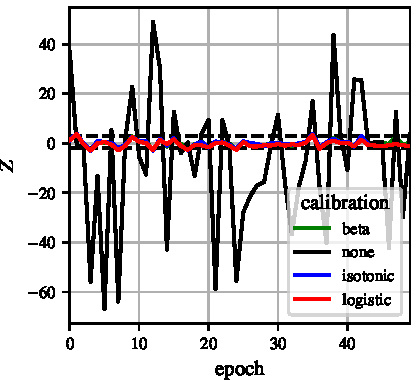
\includegraphics[scale=0.9]{figures/disc_calib_cifar.pdf}
       \caption{CIFAR-10}
       \label{fig:calibration cifar}
    \end{subfigure}
    \begin{subfigure}[b]{0.49\textwidth}
       \centering
       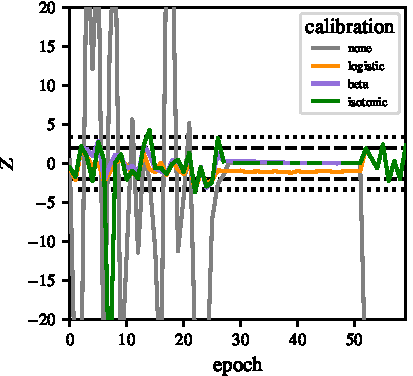
\includegraphics[scale=0.9]{figures/disc_calib_celeba.pdf}
       \caption{CelebA}
       \label{fig:calibration CelebA}
    \end{subfigure}
    \caption{{\small
    We show the calibration statistic $Z$~\eqref{eq:calib score} for the discriminator on held out data for the DCGAN\@.
    The results for CIFAR-10 are shown on the right, and CelebA on the left.
    The raw discriminator is clearly miscalibrated being far outside the region expected by chance (dashed black), and after multiple comparison correction (dotted black)\@.
    All the calibration methods give roughly equivalent results.
    CelebA has a period of training instability during epochs 30--50 which gives trivially calibrated classifiers.
    }}
    \label{fig:calibration}
\end{figure}

